% main.tex
\documentclass[12pt]{scrreprt}
\usepackage[a4paper, margin=2.5cm]{geometry}
\usepackage{xcolor}
\usepackage{listings}
\usepackage{underscore}
\usepackage[english]{babel}
\usepackage{scrlayer-scrpage}
\usepackage{setspace}
\usepackage{titlesec}
\usepackage[utf8]{inputenc}
\usepackage{placeins}
\usepackage{float}
\usepackage{graphicx}
\usepackage{caption}    % 允许子图使用 caption
\usepackage{subcaption} 
\usepackage{array}
\usepackage{colortbl}
\usepackage{booktabs}
\usepackage[bookmarks=true]{hyperref}
\usepackage{parskip}           % 段落间距
\setlength{\parskip}{0.5em}    % 紧凑段落间距
\renewcommand{\baselinestretch}{1.05} % 行距微调

% main.tex导言区
\usepackage{titlesec}
\titleformat{\chapter}[block]
{\normalfont\huge\bfseries}{\thechapter}{1em}{}
\titleformat{\section}[block]
{\normalfont\Large\bfseries}{\thesection}{1em}{}
\titleformat{\subsection}[block]
{\normalfont\large\bfseries}{\thesubsection}{1em}{}
% 保持编号与标题的经典间距
\makeatletter
\renewcommand{\@seccntformat}[1]{\csname the#1\endcsname\quad}
\makeatother

% 现代间距系统(单位:pt)
\titlespacing*{\chapter}{0pt}{25pt}{15pt}  % 上间距25pt/下间距15pt
\titlespacing*{\section}{0pt}{15pt}{7pt}
\titlespacing*{\subsection}{0pt}{10pt}{5pt}

% 确保子章节编号
\setcounter{secnumdepth}{3}
\setcounter{tocdepth}{3} % 目录显示到三级标题

% 封面字体优化
\usepackage{anyfontsize}        % 精确字体控制
\usepackage[sfdefault]{noto}   % 现代无衬线字体(需要安装Noto Sans字体)

%refers
\usepackage[style=ieee, sorting=none, backend=biber]{biblatex}
\addbibresource{re.bib}

% Hyperref配置
\hypersetup{
    pdftitle={Software Requirement Specification},
    pdfauthor={Jean-Philippe Eisenbarth},
    pdfsubject={TeX and LaTeX},
    pdfkeywords={TeX, LaTeX, SRS, Requirements},
    colorlinks=true,
    linkcolor=blue!70!black,
    citecolor=green!60!black,
    filecolor=magenta,
    urlcolor=cyan!70!black,
    linktoc=page
}

% 全局格式设置
\setstretch{1.1}
\titleformat{\chapter}[display]
{\normalfont\huge\bfseries}{\chaptertitlename\ \thechapter}{20pt}{\Huge}
\titlespacing*{\chapter}{0pt}{-30pt}{40pt}

% 自定义命令
\newcommand{\placeholder}[1]{\textcolor{gray!70}{\textlangle\,\textit{#1}\,\textrangle}}
\newcommand{\req}[2]{\item[REQ-#1:] #2} %详见设置文件

\newcommand{\myversion}{1.0}   %在这里更改文档版本

\begin{document}

% 封面
% cover.tex
\begin{flushright}
    \vspace*{1.5cm}
    \rule{0.75\textwidth}{5pt}
    
    \vspace{1.2cm}
    \fontsize{30}{28}\selectfont
    \textbf{Detailed Design}
    
    \vspace{1.5cm}
    \fontsize{14}{16}\selectfont
    for
    
    \vspace{1cm}
    \fontsize{18}{22}\selectfont
    Design and Implementation of a Lightweight \\[0.3em]
    Education Data Bay Area (E-DBA)
    
    \vspace{1.5cm}
    \fontsize{13}{15}\selectfont
    Version \myversion\ Approved
    
    \vspace{1.8cm}
    \begin{minipage}{0.7\textwidth}
    \flushright
    \fontsize{12}{14}\selectfont
    \textbf{Prepared by:} \\
    Taian Yu (FULL)\quad Yolanda Yin (FULL) \\
    Justin Zhang (FULL)\quad Aaron Liu (FULL) \\
    Steven Luo (FULL)\quad Younger Yang (FULL)
    \end{minipage}
    
    \vspace{1.2cm}
    \fontsize{14}{16}\selectfont
    Group C01
    
    \vspace{2cm}
    \today
\end{flushright}

% 目录
\tableofcontents

%迭代历史
\chapter*{Revision History}
\begin{center}
    \rowcolors{2}{gray!15}{white} % 设置表格隔行颜色
    \begin{tabular}{>{\raggedright\arraybackslash}p{3.5cm}
                    >{\raggedright\arraybackslash}p{3cm}
                    >{\raggedright\arraybackslash}p{5cm}
                    >{\centering\arraybackslash}p{2cm}}
        \toprule[1.5pt]
        \rowcolor{gray!30} % 表头颜色
        \textbf{Name} & \textbf{Date} & \textbf{Reason For Changes} & \textbf{Version}\\
        \midrule
        All Members & 9 April & Create the document & 1.0\\
        \bottomrule[1.5pt]
    \end{tabular}
\end{center}



\chapter{Overview}
\section{Project description}
This project focuses on designing the architecture for four core modules: User, Service, Data, and Others (independent objects). Each subsystem's architecture will be visually represented, along with its persistent data tables, to ensure a clear and scalable system structure.

\section{References}
SRS, UI document

\section{Design purpose}
This design aims to establish a clear modular structure to enhance the maintainability, scalability, and focus separation of users, services, data, and other subsystems. By defining dedicated subsystems to construct different architecture layers and persistent data tables, it minimizes the number of associations across subsystem boundaries, ensures efficient data flow, reduces interdependencies, and simplifies future extensions.


\chapter{Overall description}
\section{Use case diagram and class diagram}
\begin{figure}[H]
    \centering
    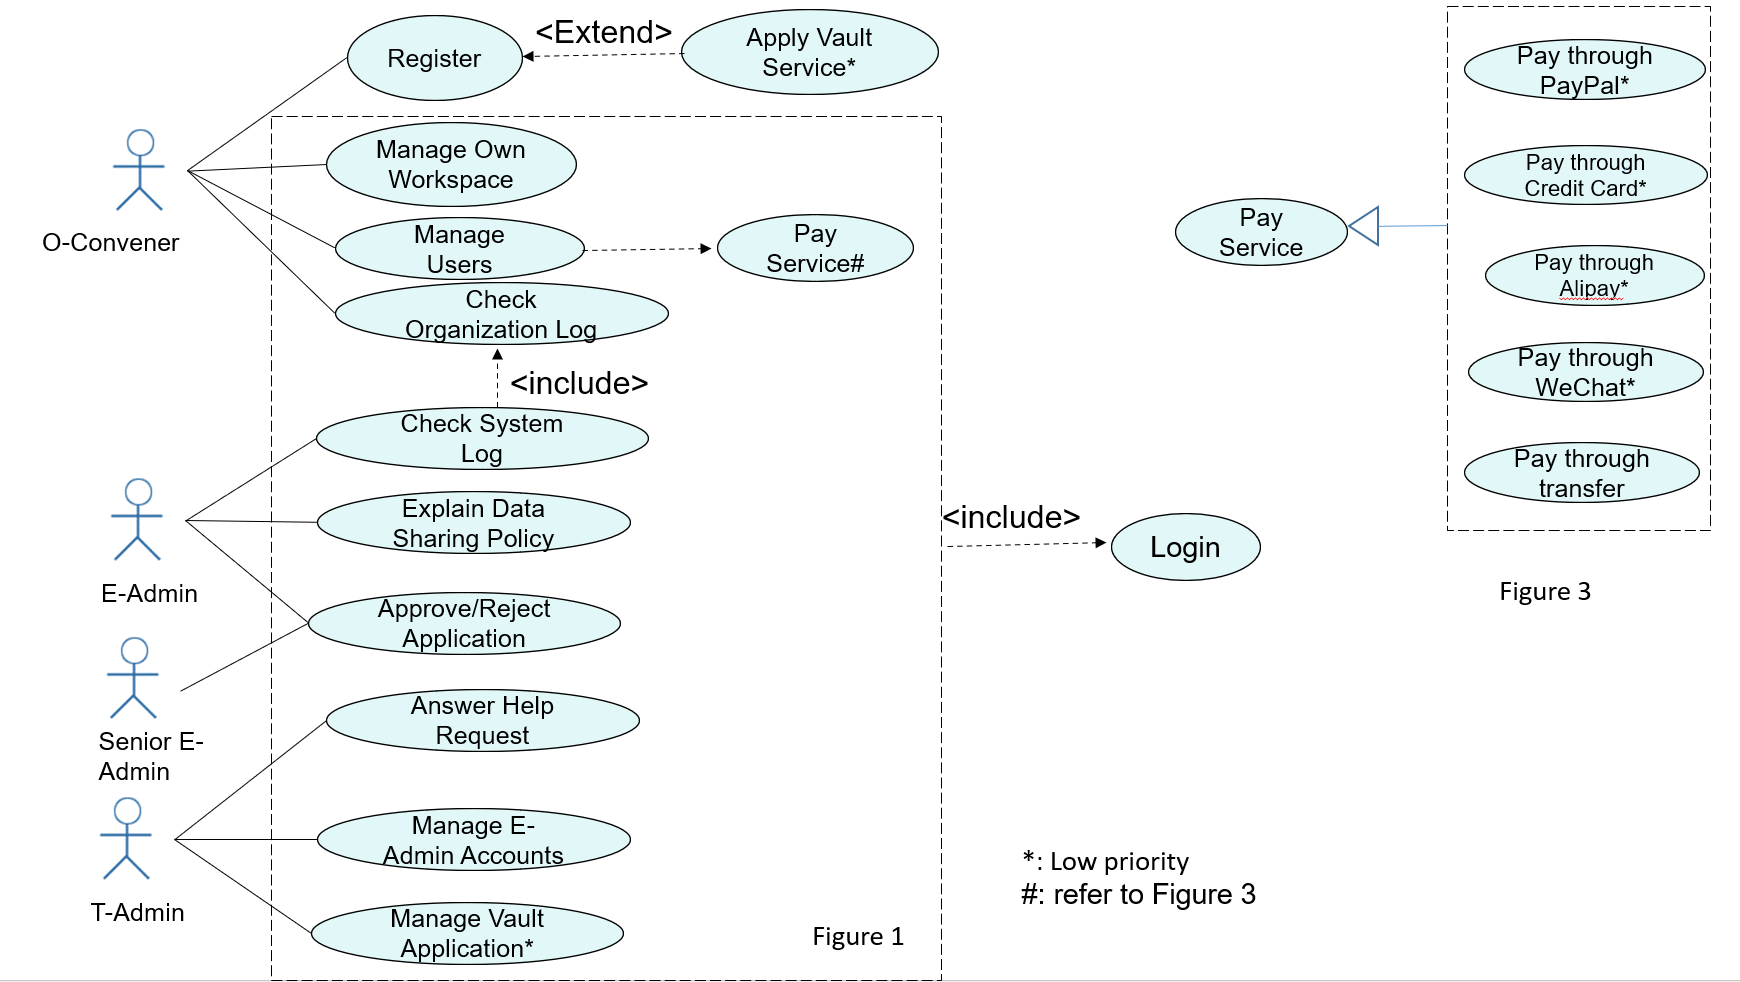
\includegraphics[width=0.75\linewidth]{picture/2-1/2-1-2.jpg}
    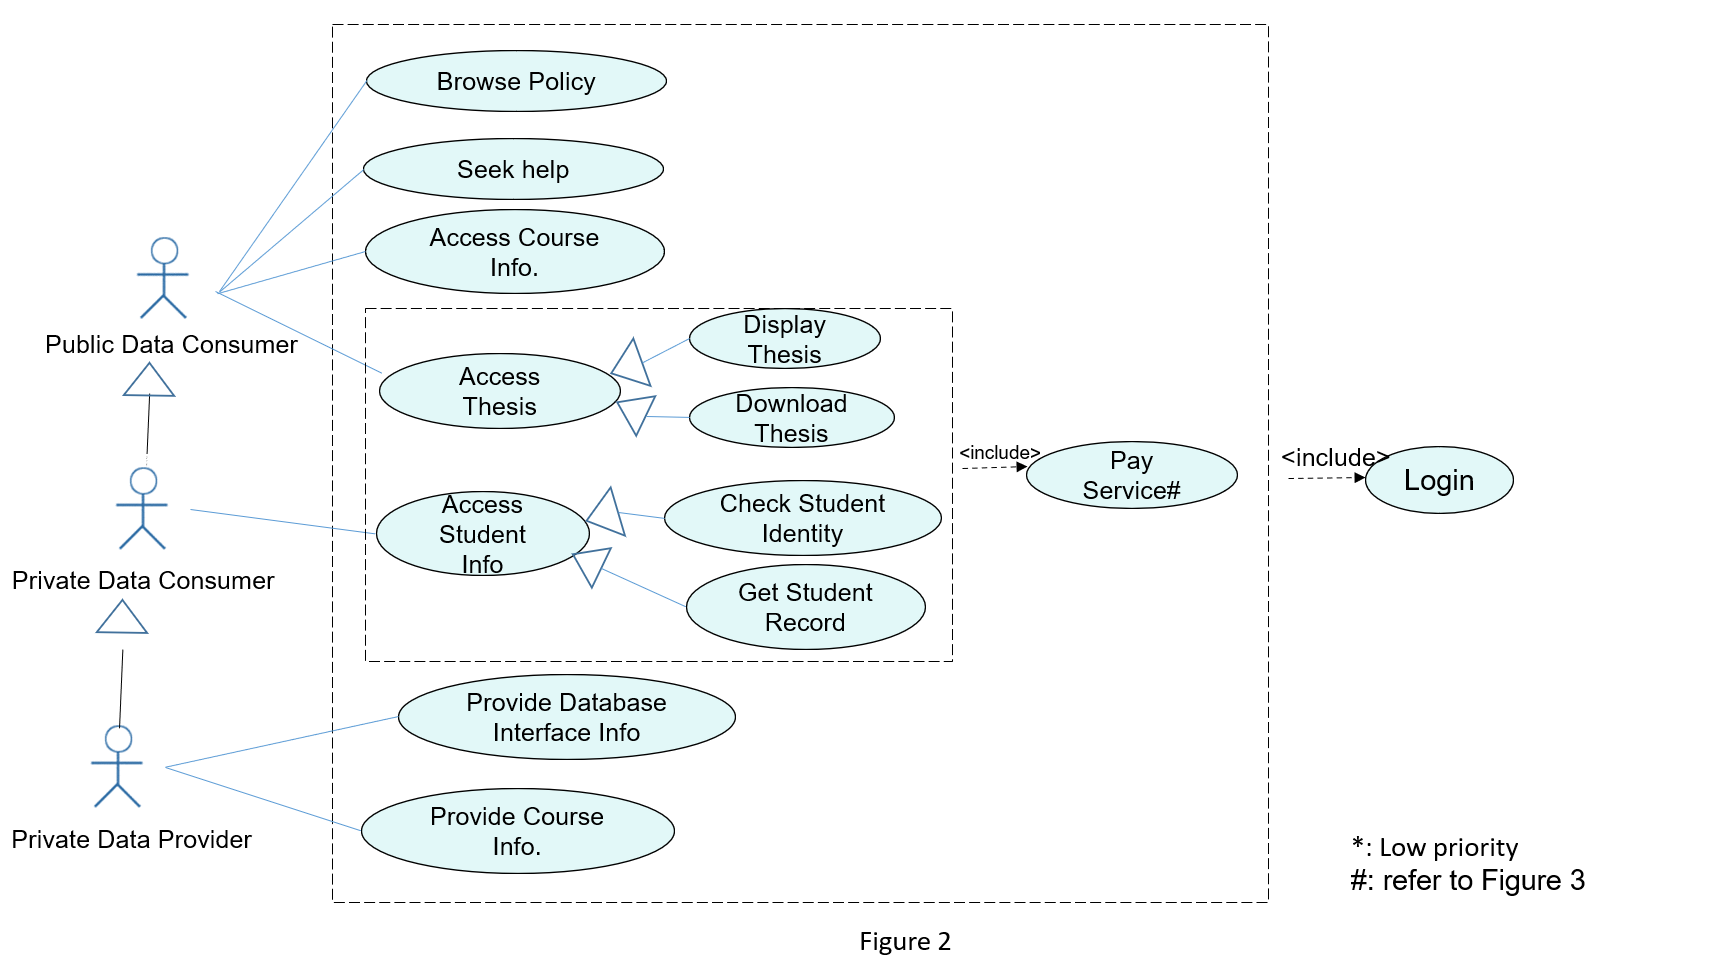
\includegraphics[width=0.75\linewidth]{picture/2-1/2-1-3.jpg}
    \caption{Use case diagram}
    \label{fig:enter-label}
\end{figure}

\begin{figure}[H]
    \centering
    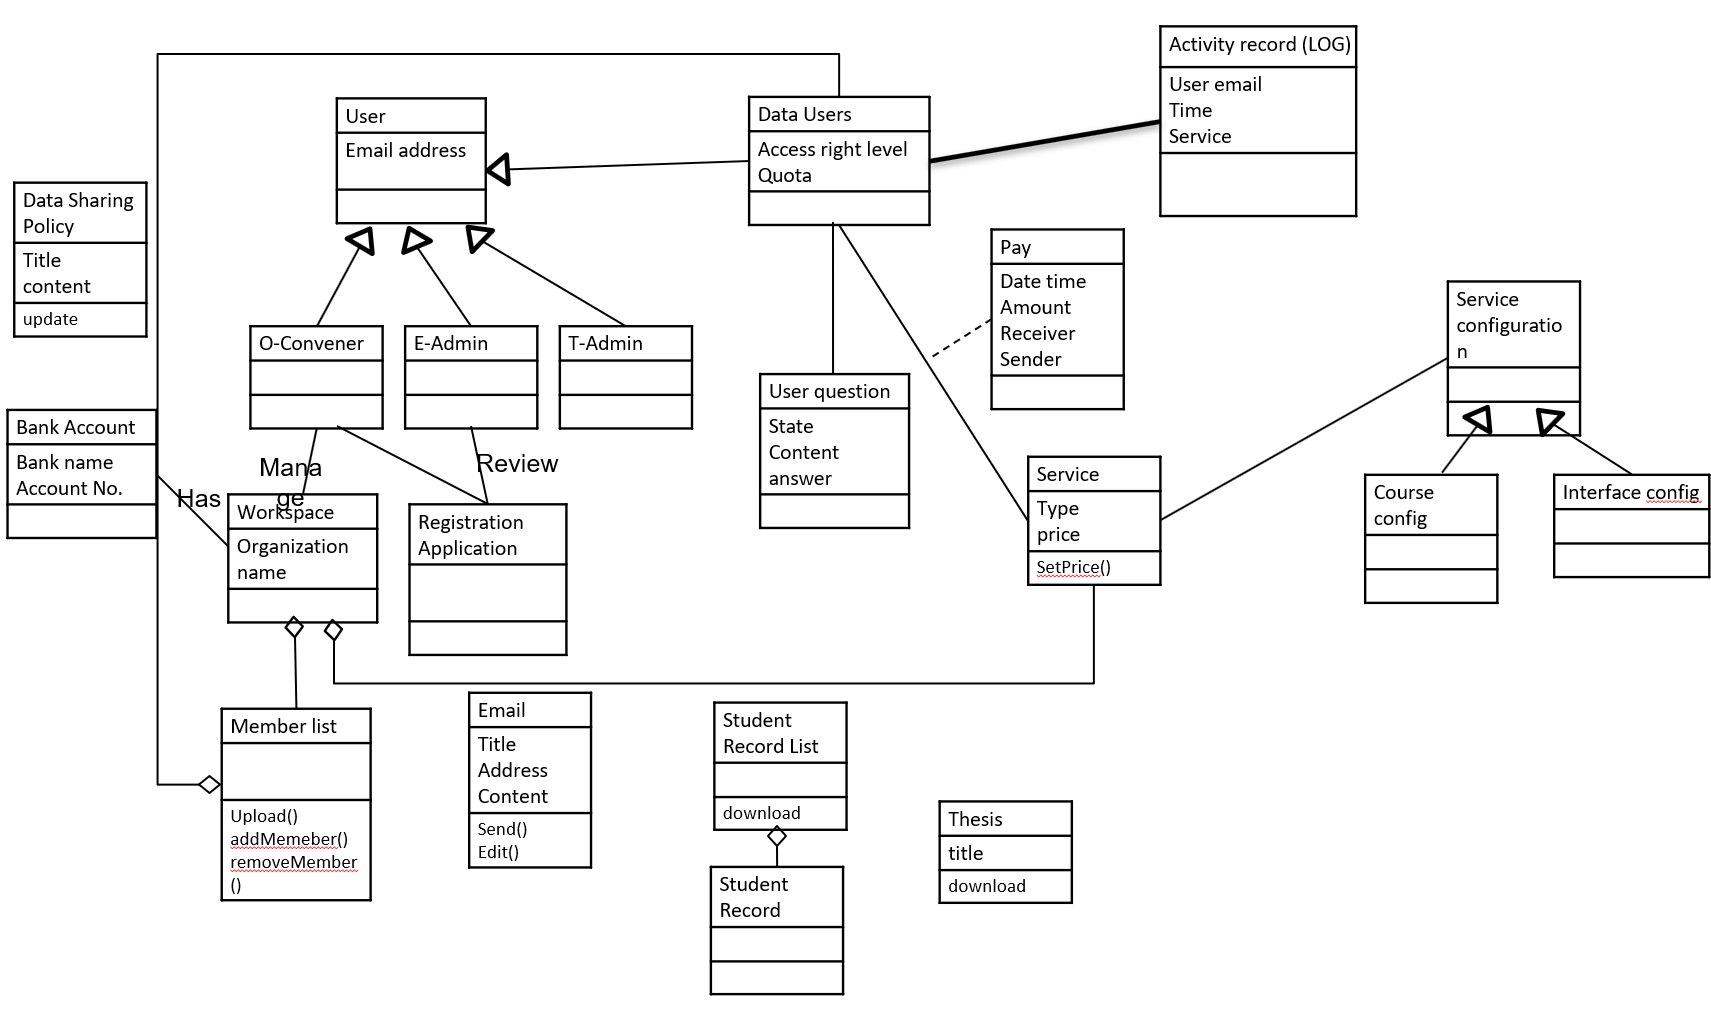
\includegraphics[width=0.75\linewidth]{picture/2-1/2-1-1.jpg}
    \caption{Class diagram}
    \label{fig:enter-label}
\end{figure}


\section{Design model}
\textbf{Layered Model} and \textbf{MVC Model} are used in this design.

The \textbf{Layered Model} divides the system into multiple levels: \textit{UserSub}, \textit{ServiceinfoSub}, \textit{DataUserSub}, and \textit{OthersSub}. The \textit{OthersSub} contains four parts: \textit{Data Sharing Policy}, \textit{Email}, \textit{Thesis}, and \textit{Student Record}. This structure helps clarify higher-level responsibilities and interactions.

The \textbf{MVC Model} consists of three subsystems: \textbf{Model}, \textbf{View}, and \textbf{Controller}. Changes in the \textbf{Model} are detected and displayed by the \textbf{View} subsystems, ensuring dynamic and responsive user interfaces.


\section{System architecture}

The architecture includes 4 subsystems. UserSub for role-based access (T-admin, E-admins, O-conveners), registration management, and organizational workspace oversight. ServiceinfoSub for course, thesis and student service configuration. DataUserSub for activity logs, user queries, and payment-service integration. OthersSub handles data policy updates, email operations, and thesis/student record storage with download capabilities.

\begin{figure}[H]
    \centering
    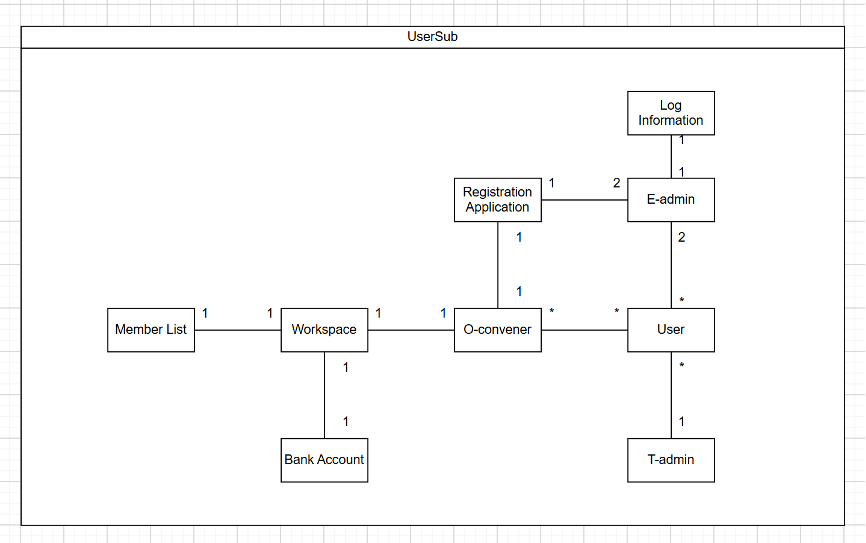
\includegraphics[width=0.75\linewidth]{picture/2-3/2-3-1.png}
    \caption{User Subsystem}
    \label{fig:enter-label}
\end{figure}

\begin{figure}[H]
    \centering
    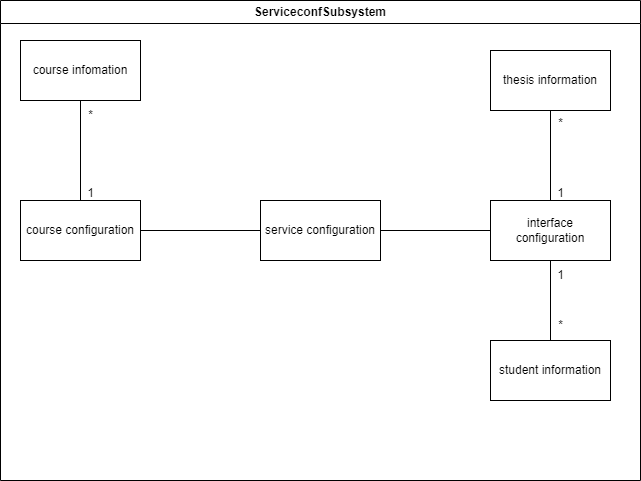
\includegraphics[width=0.75\linewidth]{picture/2-3/2-3-2.jpg}
    \caption{Service conf Subsystem}
    \label{fig:enter-label}
\end{figure}

\begin{figure}[H]
    \centering
    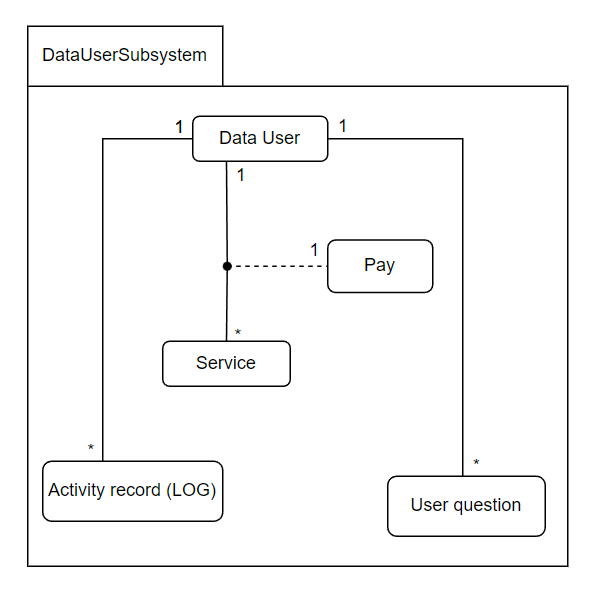
\includegraphics[width=0.75\linewidth]{picture/2-3/2-3-3.jpg}
    \caption{Data User}
    \label{fig:enter-label}
\end{figure}

\begin{figure}[H]
    \centering
    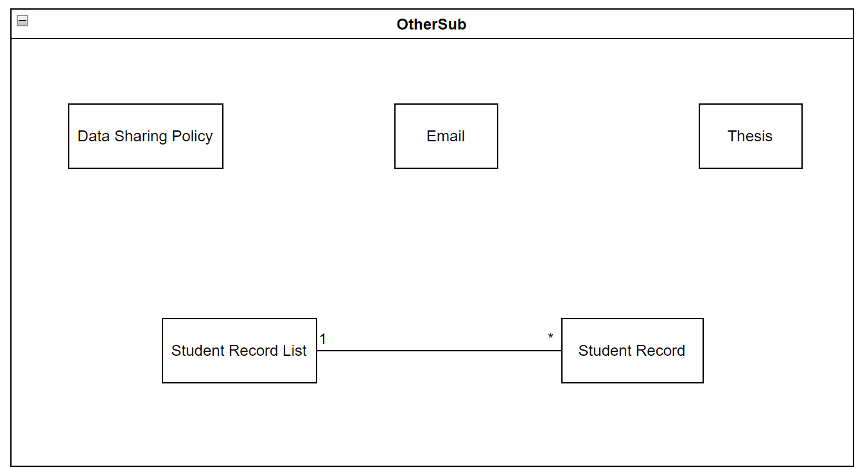
\includegraphics[width=0.75\linewidth]{picture/2-3/2-3-4.png}
    \caption{Other Sub}
    \label{fig:enter-label}
\end{figure}


\chapter{System architecture}

\section{User Subsystem}

\begin{figure}[H]
    \centering
    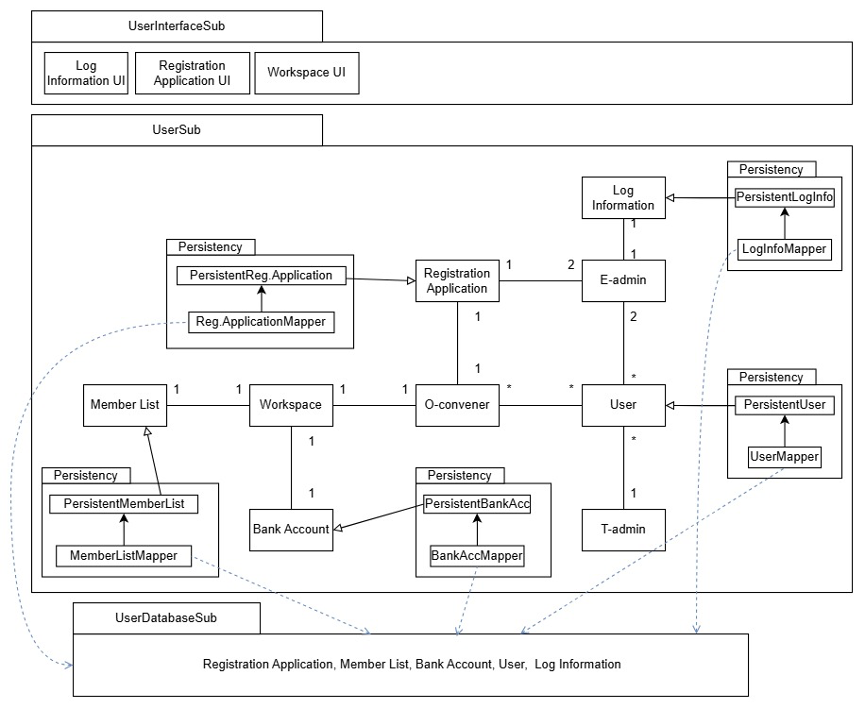
\includegraphics[width=0.75\linewidth]{picture/3-1/3-1-1.png}
    \caption{User Subsystem}
    \label{fig:enter-label}
\end{figure}

\subsection{Description}

The system has the defualt User component which is then further classified into T-admin, E-admins or O-convener. E-admins can check Log information that records all user activity in the E-DBA, and can review Registration Applications submitted by O-conveners of each organization. O-conveners can submit Registration Applications that includes information of their organization for review, and can manage the Workspace belonging to that organization. The Workspace of each organization maintains a List of Members that can access the services provided by the Workspace and also has a Bank Account linked to it.

\subsection{Database}
\begin{figure}[H]
    \centering
    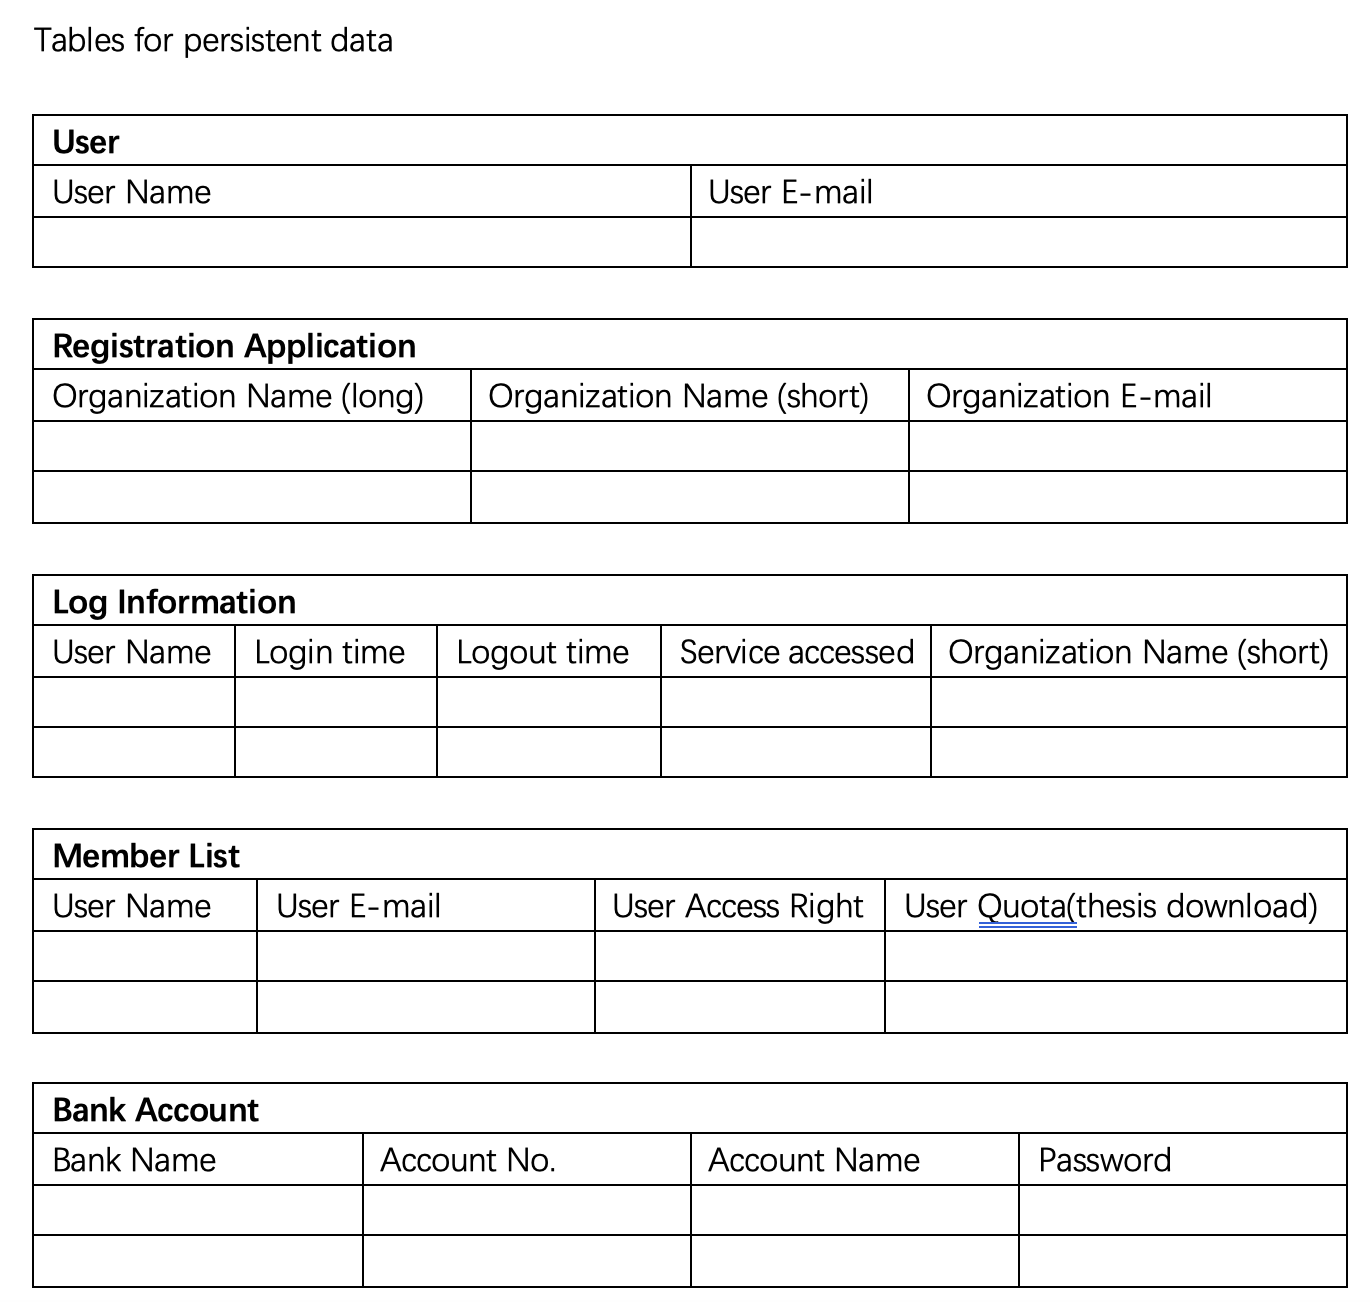
\includegraphics[width=0.75\linewidth]{picture/3-1/3-1-2.png}
    \caption{Database}
    \label{fig:enter-label}
\end{figure}

\section{Service conf Subsystem}

\begin{figure}[H]
    \centering
    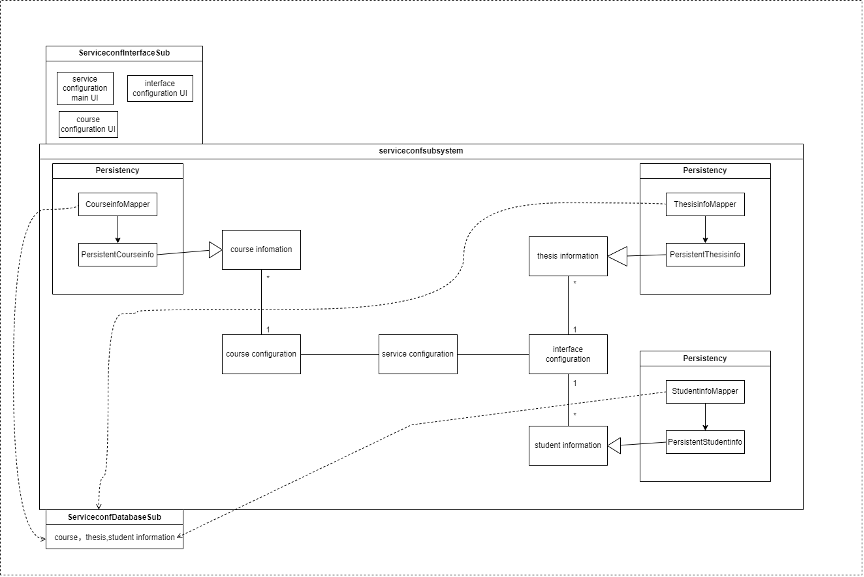
\includegraphics[width=0.75\linewidth]{picture/3-2/3-2-1.png}
    \caption{Service conf Subsystem}
    \label{fig:enter-label}
\end{figure}

\subsection{Description}

This subsystem is divided into course configuration and interface configuration. The Private data provider can edit the course information service through this course configuration page. At the same time, he can configure and share thesis information and student information service through the interface configuration page.

\subsection{Database}
\begin{figure}[H]
    \centering
    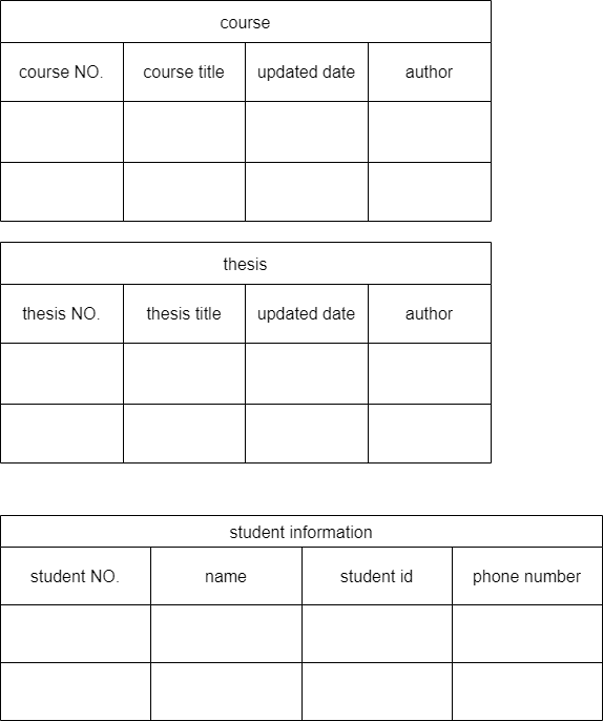
\includegraphics[width=0.75\linewidth]{picture/3-2/3-2-2.png}
    \caption{Database}
    \label{fig:enter-label}
\end{figure}

\section{Data User}

\begin{figure}[H]
    \centering
    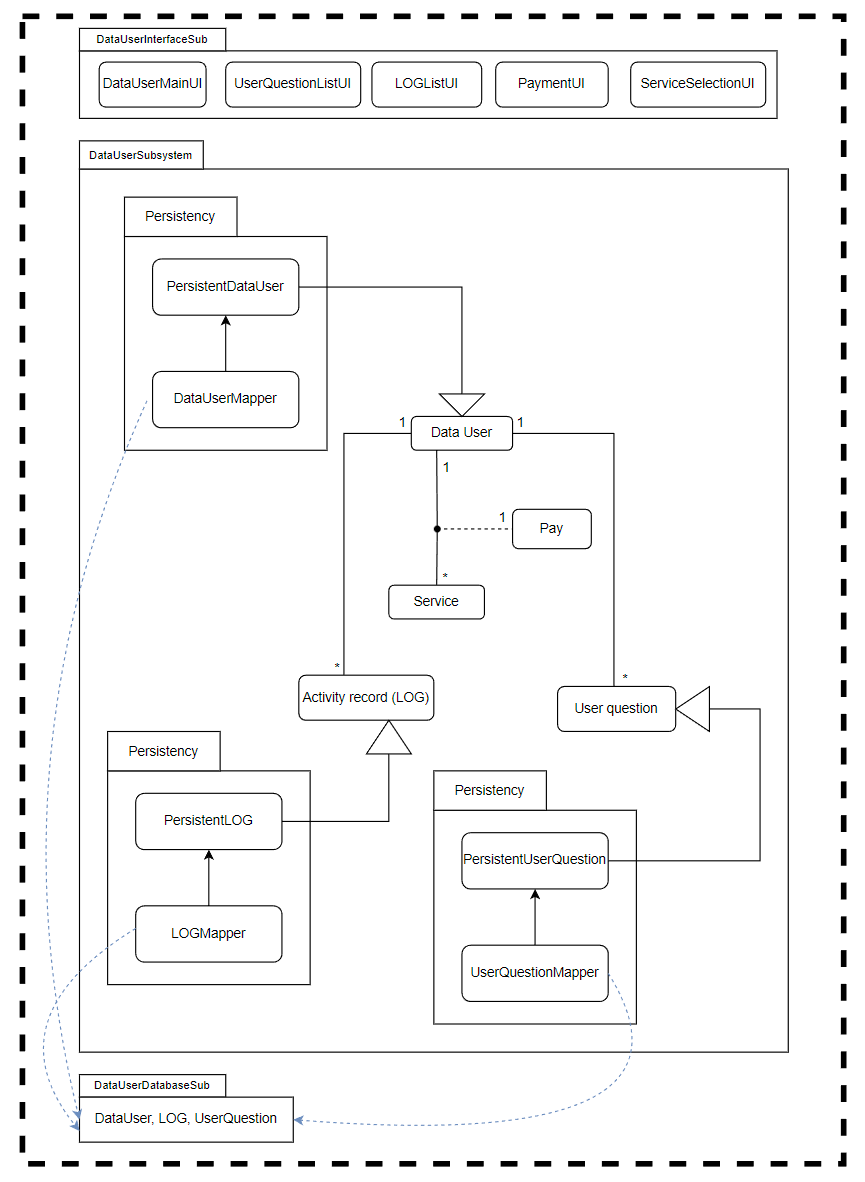
\includegraphics[width=0.75\linewidth]{picture/3-3/3-3-1.jpg}
    \caption{Data User}
    \label{fig:enter-label}
\end{figure}

\subsection{Description}

Data User is the beginning of the subsystem, it can access activity record, user question, pay and service. Activity record, which is called LOG either, can store the data of the history of happened event. User question is a list that data user can see the questions that users ask. Service can be obtained after payment.

\subsection{Database}
\begin{figure}[H]
    \centering
    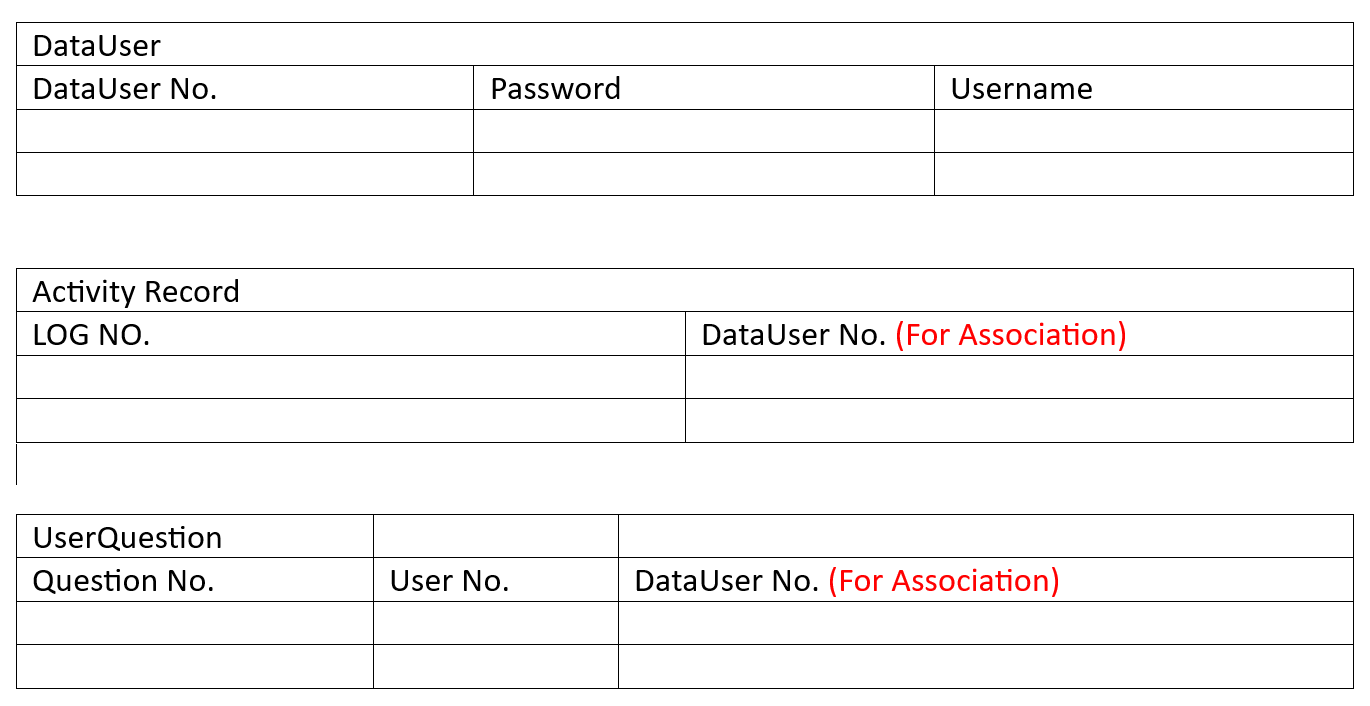
\includegraphics[width=0.75\linewidth]{picture/3-3/3-3-2.jpg}
    \caption{Database}
    \label{fig:enter-label}
\end{figure}

\section{Other Sub}

\begin{figure}[H]
    \centering
    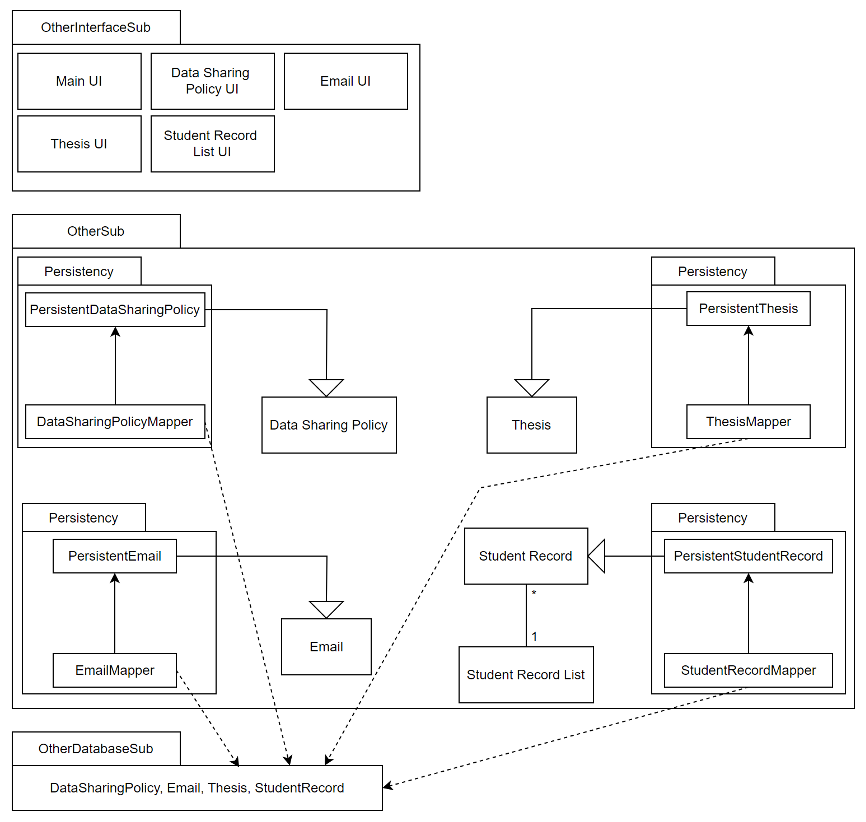
\includegraphics[width=0.75\linewidth]{picture/3-4/3-4-1.png}
    \caption{Other Sub}
    \label{fig:enter-label}
\end{figure}

\subsection{Description}

The other-subsystem contains 4 parts, data sharing policy, email, thesis and student record, the data sharing policy has title and content while it could be updated, the email has title, address, content while it could be sent or edit, the thesis has title, the student record belongs to a student record list while both thesis and student record could be downloaded. 

\subsection{Database}
\begin{figure}[H]
    \centering
    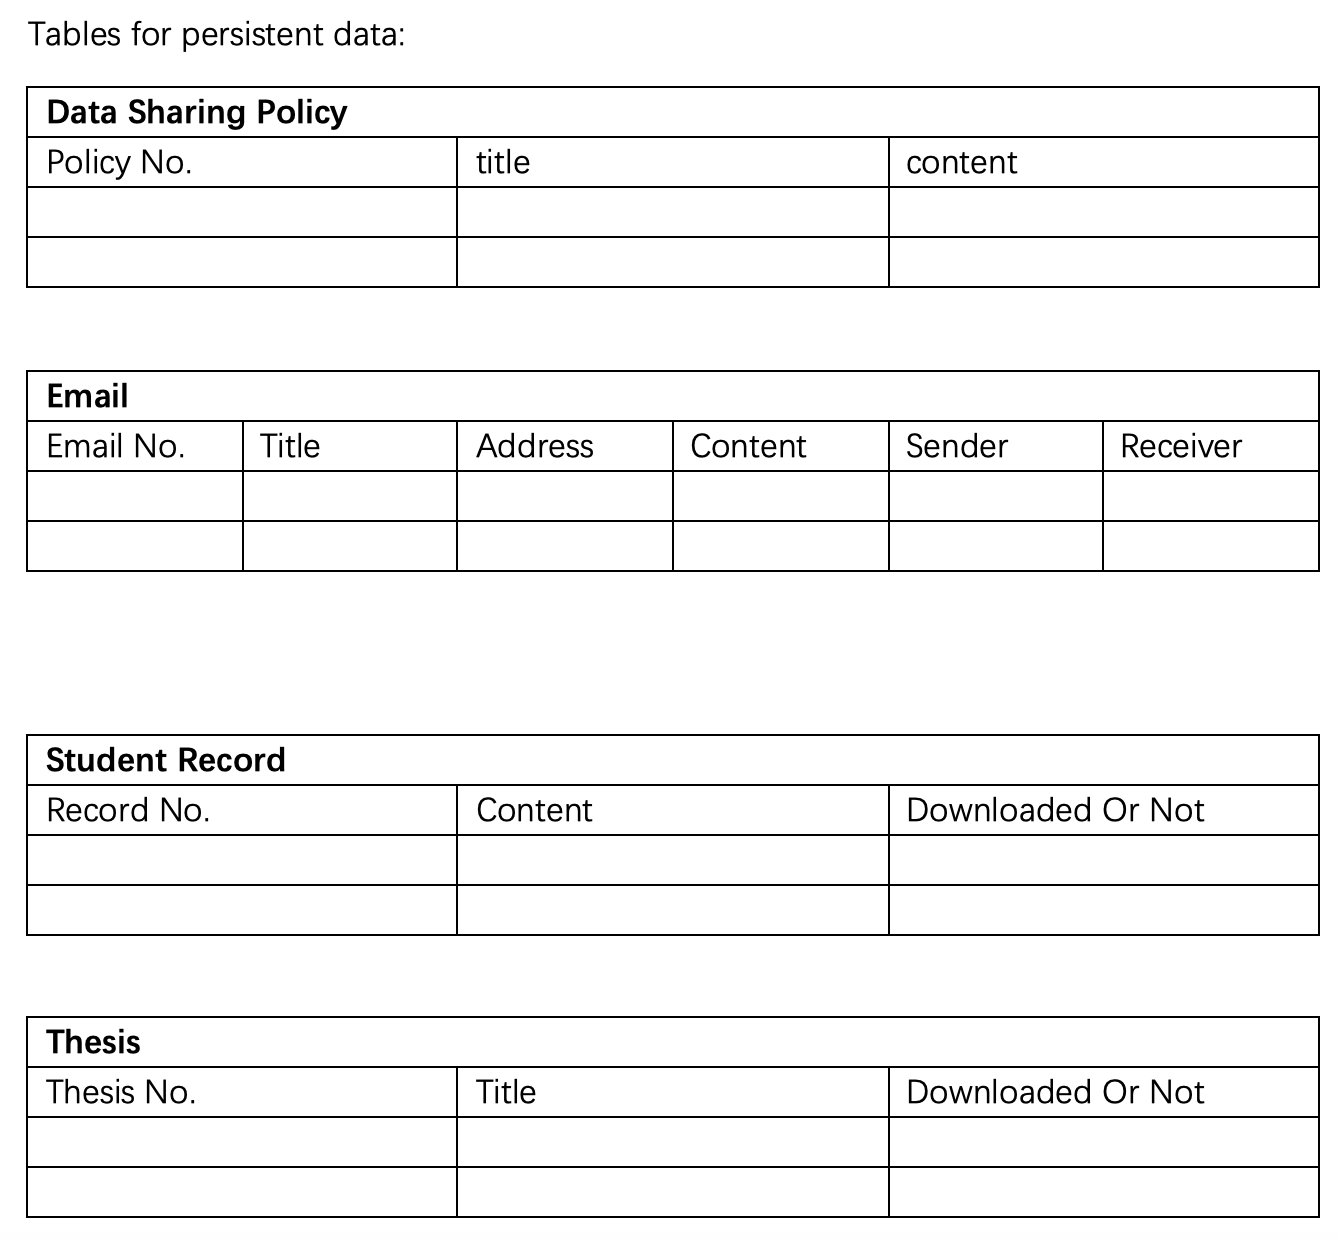
\includegraphics[width=0.75\linewidth]{picture/3-4/3-4-2.png}
    \caption{Database}
    \label{fig:enter-label}
\end{figure}

\chapter{Assessment}

\section{Stability}
\textbf{Low Coupling}
The system employs a layered architecture, isolating UI components (e.g., PaymentUI) from persistence logic (e.g., CourseInfoMapper), minimizing ripple effects during modifications. Persistence layers focus on specific data domains, reducing dependencies.  

\textbf{High Cohesion }
Modules like UserSub (user registration) and DataUserSubsystem (log management) group related logic, while dedicated UIs (e.g., PaymentUI) partition business functions, ensuring focused responsibilities and consistency. 

\section{Reusability}
The system shows stable interfaces between layers, enabling components to be reused without modifications. The UI layer (e.g., PaymentUI, ServiceSelectionUI) interacts with backend logic via well-defined contracts, allowing UI replacements without disrupting underlying operations. Persistence components like CourseInfoMapper and PersistentLOG encapsulate domain-specific data handling, ensuring their interfaces remain consistent even when reused across subsystems (e.g., integrating user registration logic from UserSub into other modules). Modular design (e.g., DataUserSubsystem for logs) further supports reusability by grouping cohesive functionalities into self-contained units.

\section{Scalability} 
The system’s layered architecture and modular design (e.g., isolated UI, persistence layers) support vertical scaling (e.g., enhancing database performance). However, horizontal scaling (e.g., distributing workloads) may require decoupling tightly bound components like redundant numbered modules. Streamlining dependencies and standardizing interfaces would further improve flexibility for future expansion.


\chapter{Alternative design (optional)}
None

\chapter{More considerations}
None

\chapter{Appendix}
None

% If there are any changes to the teacher's requirements, these will be copied to where they should be.
 
\nocite{*}
\printbibliography[heading=bibintoc]

\end{document}